\newpage
 \appendix
 \renewcommand\appendixname{Anexo}
 \setcounter{chapter}{0}
 \renewcommand\thechapter{\Alph{chapter}}

 % \usepackage[spanish]{babel}
 % \usepackage[T1]{fontenc}
 % \usepackage{times}
 % \usepackage[utf8]{inputenc}
 
 % \usepackage{spverbatim}
 % \usepackage{amsmath}
 % \usepackage[usenames]{color}
 
 % \usepackage{graphicx}
 % \usepackage{subfigure}
 % \usepackage[utf8]{inputenc} 
 
 % \usepackage[Conny]{fncychap} \ChTitleVar{\vspace{1.5cm}\centering\Huge\rm\bfseries} \ChNameVar{\vspace{1.5cm}\centering\Huge\rm\bfseries}

 \newpage
 
\chapter{Guía de Implementación para MINSOC}

 %\section{GUÍA DE IMPLEMENTACION DE MINSOC}

	\section{\textcolor{orange}{Introducción}}

Para utilizar el procesador OR1200 OpenRISC se usan una serie de periféricos básicos los cuales se comunican a través de un bus wishbone, creando un system-on-chip (SoC). 

El proyecto MinSoc es un un SoC básico que  contiene el procesador OR1200, un modulo de depuración basado en una interfaz JTAG, un modulo de RAM  interna, un modulo UART y Ethernet.

El SoC permite cargar un pequeños programas en la memoria interna usando el Cable USB  Xilinx Platform que utiliza uno de los puertos de acceso TAP (Test Access Port) JTAG. El procesador ejecuta el programa desde la memoria interna, usando como salida los modulos UART y Ethernet. 

\begin{figure}[h!]
 \begin{center}
  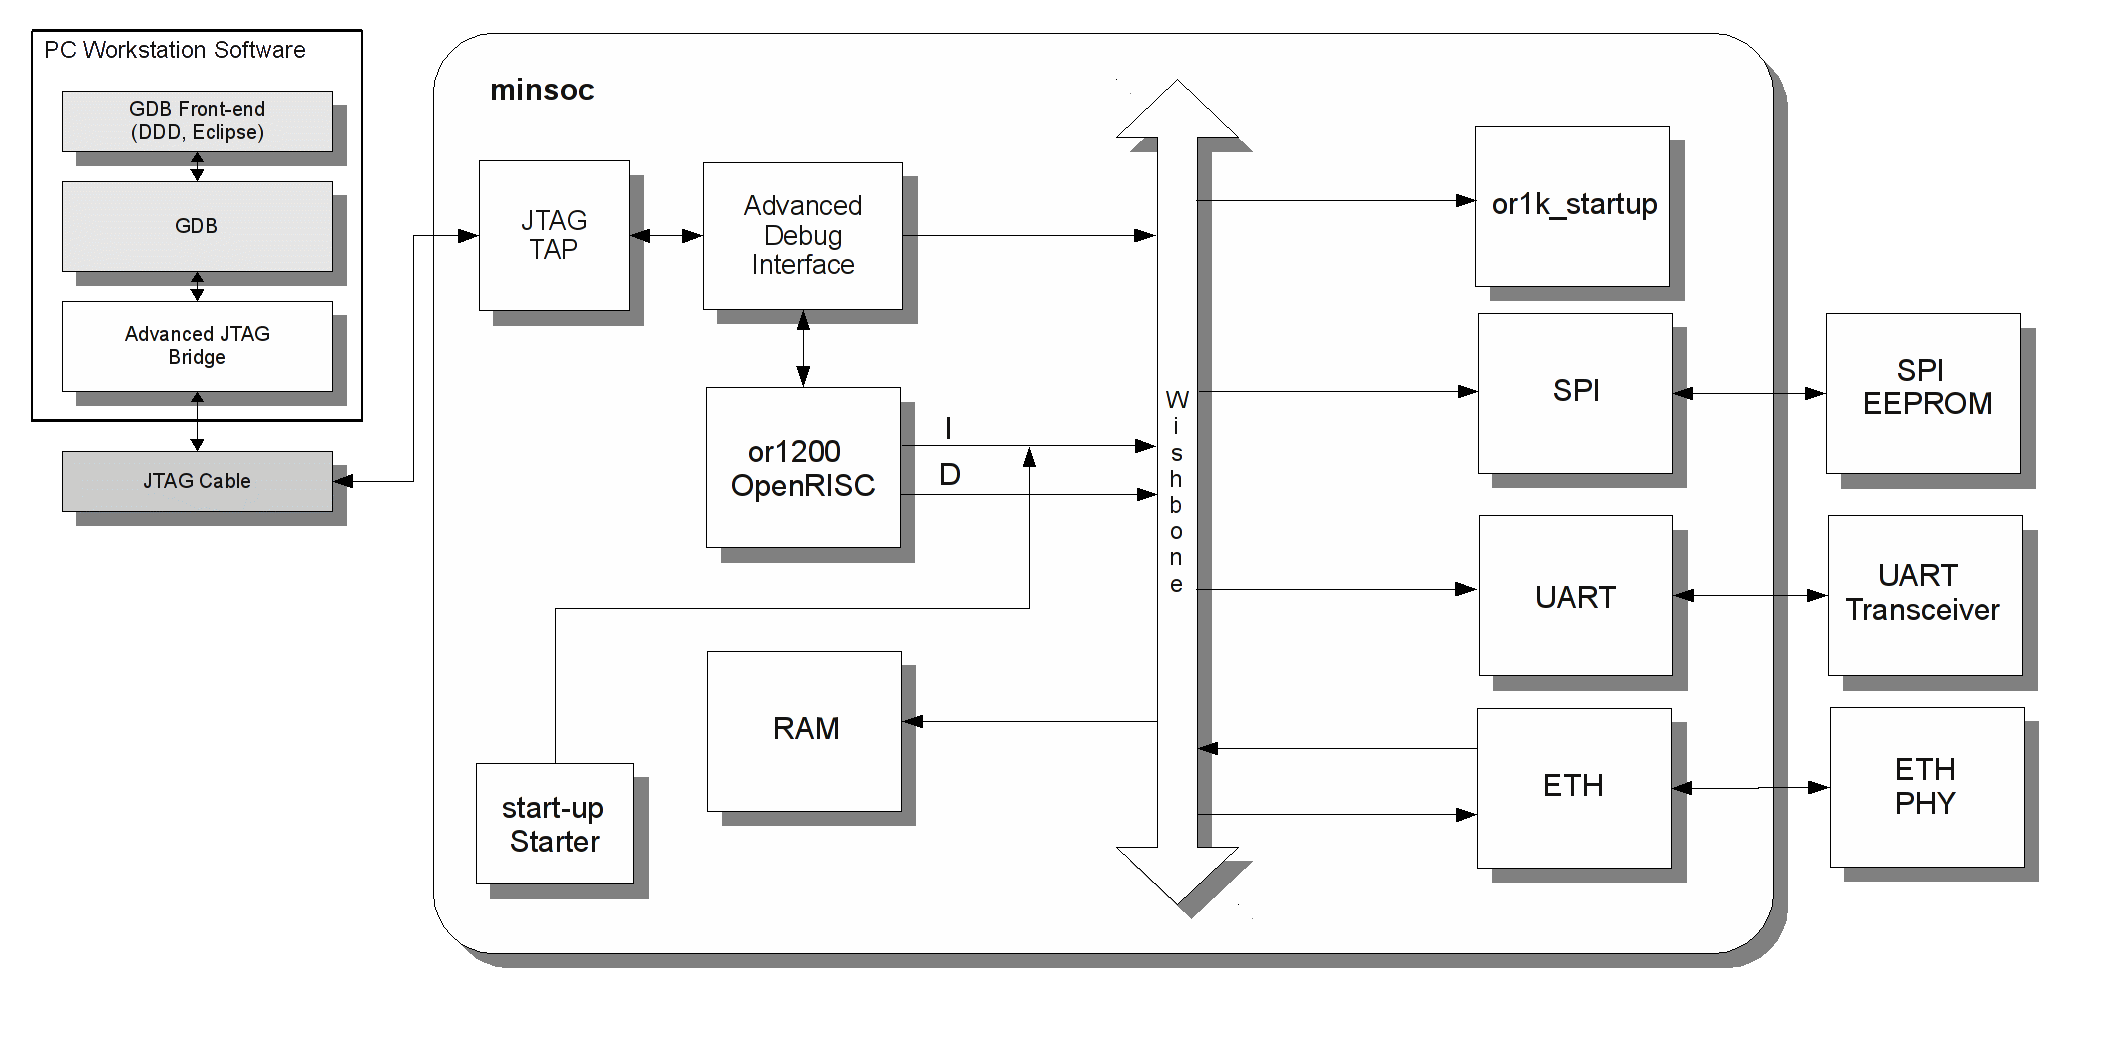
\includegraphics[width=1\textwidth,keepaspectratio=true]{./images/minsoc}
  \caption{Arquitectura MinSoc}
  \label{fig:esquema}
 \end{center}
\end{figure}

La guía práctica, está divida en dos partes principales: 

En la primera parte se detalla, principalmente, los pasos a seguir para poder configurar e implementar un SoC en la placa de desarrollo XILINX XtremeDSP Starter Platform Spartan 3A DSP 1800.


En la segunda parte se presenta la compilación cruzada con las herramientas de GNU para OpenRisc de un software de prueba, cargado a través del sistema de Debug Advanced con salida por modulo UART al puerto serie de la PC .

	%En la tercera parte se explica, además, lo problemas y soluciones para la implementación en el kit XILINX XtremeDSP Starter Platform Spartan 3A DSP 1800.

\newpage
\section{\textcolor{orange}{Objetivos del Proyecto MinSoc}}

La idea del proyecto es ofrecer un SoC sintetizable que sea  compatible con cualquier placa con una FPGA sin necesidad de modificaciones en su código RTL. El proyecto posee un depurador del sistema Debug Advanced,  el que permiten depurar el sistema con los mismos cables utilizados para la configuración de la FPGA. 

\section{\textcolor{orange}{Convenciones tipográficas}}

A largo de esta guía se utiliza la siguiente convención tipográfica: 

\begin{itemize}
\item Texto plano: se usa para indicar el contenido de un archivo, porciones de código y la salida que se muestra por consola al ingresar un comando.
\item Texto plano en negrita : se usa para indicar aquello que se ingresa por consola, usualmente, un comando. 
\item Texto plano entre corchetes angulares>: se usa para hacer referencia a un directorio. 
\item user@dist: se usa para indicar el prompt de la consola, tanto del host como del target. 
\end{itemize} 
 
Por ejemplo, la siguiente línea muestra que se ejecuta el comando ls en el directorio rootfs (que a  su vez se encuentra dentro del directorio\_ejemplo), en un host cuyo usuario es user y utiliza una distribuciòn dist de Linnux:


\begin{lstlisting}[breaklines]
user@dist:<directorio_ejemplo>/rootfs$ ls
\end{lstlisting}

\section{\textcolor{orange}{Requerimientos previos}}

 Para poder llevar a cabo la instalación de las herramientas de diseño de Hardware,sintetizar, implementar y efectuar debuging  del proyecto MinSoc en el kit de desarrollo, se necesita:

\begin{itemize}
\item Host de desarrollo con Ubuntu (12.4, preferentemente).
\item XILINX XtremeDSP Starter Platform Spartan 3A DSP 1800.
\item Xilinx ISE 14.2 con el directorio bin agregado al PATH.
\item Instalación del derive para el cable Platform Cable USB II.
\item Adaptador RS-232 a USB.
\item Emulador de consola.
\item Conexión a internet para descarga de paquetes.

\end{itemize} 

\newpage

\section{\textcolor{orange}{Dependencias}}

La instalación de las herramientas involucran la configuración previa de ciertas aplicaciones (como el tar) y la instalación de algunos paquetes.
Las siguientes son las dependencias necesarias para poder ejecutar el script de instalación del proyecto MinSoc

wget

svn

bzip2

tar

sed

patch

gcc

make

makeinfo

libncurses\-dev

flex

bison

libz\-dev 


 
\section{\textcolor{orange}{Instalación }}

El script de instalación funciona bajo cualquier Linux. Otros sistemas no son compatibles.

El script de instalación instala la cadena de herramientas GNU para OpenRISC, el adv\_ jtag\_ bridge para el software de carga y depuración y Icarus Verilog para la simulación del sistema. También descarga MinSoC y lo configura.
 

\subsection{\textcolor{orange}{Descarga de el script de instalación:}}

\begin{lstlisting}[breaklines]
 user@dist:~/$svn export http://opencores.org/ocsvn/minsoc/minsoc/tags/release-1.0/utils/
setup setup
\end{lstlisting}

\subsection{\textcolor{orange}{Ejecute el script de instalación}}

\begin{lstlisting}[breaklines]
user@dist:<directorio_de descarga_release-1.0>/minsoc/utils/setup$ minsoc-install.sh
\end{lstlisting}

La ejecución de este script requiere del usuario la ruta en la que se va a instalar el sistema.Por ejemplo:

\begin{lstlisting}[breaklines]
/home/user/Escritorio/minsoc
\end{lstlisting}

El sistema tiene la siguiente estructura de directorio después de ser ejecutado: 
\begin{lstlisting}[breaklines]
install_path/
	download/
	 tools/
 	 minsoc/
\end{lstlisting}

Todas las herramientas necesarias están instaladas en le directorio tools. Los paquetes descargados se encuentran en download y son compilados allí. El Advanced JTAG Bridge se agrega automáticamente a la ruta minsoc/rtl/verilog/adv\_debug\_sys/Software/adv\_jtag\_bridge  y también es compilado allí. 

Al final del script están incluidas las rutas de los binarios de las herramientas y los  binarios de el Toolchain de GNU en el directorio /home/user/.bashrc
 
Después de la correcta ejecución de el script, se pueden eliminar el directorio download y todo quedara instalado.

Antes de utilizar el sistema, se tiene que reiniciar el shell o cargar las nuevas variables de entorno ejecutando la linea de comando:

\begin{lstlisting}[breaklines]
user@dist:<directorio_de descarga_release-1.0>/minsoc/utils/setup$ sourece /home/user/.bashrc
\end{lstlisting}

\section{\textcolor{orange}{Síntesis}}

\subsection{\textcolor{orange}{Configuración de la placa especifica para la síntesis}}
Dentro del subdirectorio minsoc/backend/ se busca la placa en la que queremos implementar el proyecto MinSoc. Nos dirigimos al directorio correspondiente y ejecutamos el script de configuración.

\begin{lstlisting}[breaklines]
user@dist:<directorio_de_instalación>$cd minsoc/backend/spartan3a_dsp_kit 
user@dist:<directorio_de_instalación>/minsoc/backend/spartan3a_dsp_kit $./configure 
\end{lstlisting}

El sistema está configurado ahora, se puede proceder a la síntesis.

\subsection{\textcolor{orange}{Generación del .Bit}}

MinSoC utiliza un archivo Makefile para sintetizar su diseño. El sistema para sintetizar se encuentra en el subdirectorio minsoc/syn/xilinx. Una vez realizada la síntesis se creara el archivo .bit necesario para configurar la FPGA.

\begin{lstlisting}[breaklines]
user@dist:~<directorio_de_instalación>/minsoc/syn/xilinxt$make all
\end{lstlisting}

Después de que se ha generado el archivo de .bit, se cargar el archivo a la FPGA utilizando la herramienta del proveedor para este propósito como es en este caso iMPACT o mediante un herramienta Open Source llamada xc3sprog. 

\section{\textcolor{orange}{Complilacion de un Software para OpenRisc}}

Para compilar cualquier aplicación que vaya a ser ejecutada en el SoC con un micro OpenRisc, se necesita utilizar un compilador cruzado en este caso es el or32-elf-gcc que se encuentra incluido en el PATH por medio de el script de instalación minsoc-install.sh.

\begin{lstlisting}[breaklines]
user@dist:~<directorio_de_instalación>/minsoc/sw/uart$ make all
\end{lstlisting}
 
El comando make construye todas las librerías y archivos binarios, en este caso se creará el binario uart.or32 que sera cargado y debuging en el SoC.
 

Si tiene dudas sobre alguno de los comando/herramientas utilizados en esta sección se aconseja consultar al manual correspondiente a su terminal.


\section{\textcolor{orange}{Carga y Debugging de Software}}


Para conectar con éxito el TAP del SoC que contiene el micro OpenRISC , se debe copiar los archivos BSDL de todos los dispositivos conectados a la cadena de JTAG a un directorio conocido (por ejemplo /home/user/bsdl).Luego debe colocarse, el directorio como argumento al llamar adv\_jtag\_bridge, adv\_jtag\_bridge-b /home/user/bsdl.

\begin{enumerate}

\item Conecte el cable JTAG al TAP.
\item Inicio adv\_jtag\_bridge

\begin{lstlisting}[breaklines]
user@dist:~/$sudo adv_jtag_bridge -b<directorio_bsdl> xpc_usb 
\end{lstlisting}

Por ejemplo:

\begin{lstlisting}[breaklines]
user@dist:~/$sudo adv_jtag_bridge -b /home/user/bsdl xpc_usb 
\end{lstlisting}

El parametro -b <directorio\_bsdl> de adv\_jtag\_bridge para indicar el directorio donde obtener los archivos BSDL.

Al ser ejecutado en linux y utilizar cables xpc\_usb tiene que ejecutarse como superusuario.


\item Una vez que el programa se encuentre en funcionamiento se debe abrir otro terminal (por ejemplo gtkterm).
\item Configuramos el puerto a un puerto serie conectado a la placa.
\item Configuramos el bitrete a 115200.

\item Se inicia gdb y se carga el firmware de ejemplo compilado previamente para OpenRisc.

\item 
\begin{lstlisting}[breaklines]
user@dist:~/<directorio_de_instalación>minsoc/sw/uart$ or32-elf-gdb uart.or32
target remote :9999
load
set $pc=0x100
c
\end{lstlisting}

\item Dentro de gtkterm debería haber aparecido "Hello World". 

\end{enumerate}

%\newpage
%\section{\textcolor{orange}{Problemas y soluciones}}

\newpage

\section{\textcolor{orange}{Acrónimos y abreviaturas}}

\begin{table}[!h]
\begin{center}
\begin{tabular}{|c|c|}
\hline
\rowcolor[RGB]{255,127,0} Abreviatura & Significado en ingles \\
\hline
FPGA & Field Programmable Gate Array  \\
\hline
TAP & Test Access Port  \\
\hline
\hline
BSDL & Boundary Scan Description Language  \\
\hline
\hline
JTAG & Joint Test Action Group  \\
\hline
\hline
SoC & System on Chip\\
\hline
\hline
RAM & Andom Access Memory \\
\hline
\hline
USB & Universal Serial Bus  \\
\hline
\hline
DSP& Digital Signal Processing \\
\hline
\hline
RTL & Register transfer level \\
\hline
\hline
GNU & GNU is not Unix\\
\hline
\end{tabular}
\end{center}
\end{table}

\newpage

\section{\textcolor{orange}{Bibliografía}}
\subsection{\textcolor{orange}{Documentos}}
\begin{itemize}
\item Spartan\-3A DSP Starter Platform User Guide\url{http://www.xilinx.com/support/documentation/boards_and_kits/ug454_sp3a_dsp_start_ug.pdf}.
\item Matthew Hicks. University of Illinois at Urbana\-Champaign. "guideTop".  
\end{itemize} 
\subsection{\textcolor{orange}{sitios web}}
\begin{itemize}
\item \url{http://www.minsoc.com/}
\item \url{http://opencores.org/or1k/OR1200_OpenRISC_Processor}
\item\url{http://www.xilinx.com/products/boards-and-kits/HW-SD1800A-DSP-SB-UNI-G.htm}

\end{itemize} 



 \newpage
 \chapter{Guía Básica de Implementación para ORPSoC}

 \section{Introdución}
Este proyecto implementa una plataforma para el desarrollo OpenRISC. Proporciona un SoC de referencia, para la prueba y el desarrollo de procesadores OpenRISC.

 \section{Descarga del ORPSoC}
La el código fuente RTL, el software de prueba y scripts de instalación pueden ser descargados del repositorio svn del proyecto OpenRISC. Los archivos pueden descargados con el siguiente comandos.

\begin{lstlisting}[breaklines]
 usuario@usuario-desktop:~/$  svn co http://opencores.org/ocsvn/openrisc/openrisc/trunk/orpsocv2
\end{lstlisting}

Después de descomprimir el archivo descargado para la instalación ORPSoC se parece a esto ~\ref{fig:esquema} 

\begin{figure}[h!]
 \begin{center}
  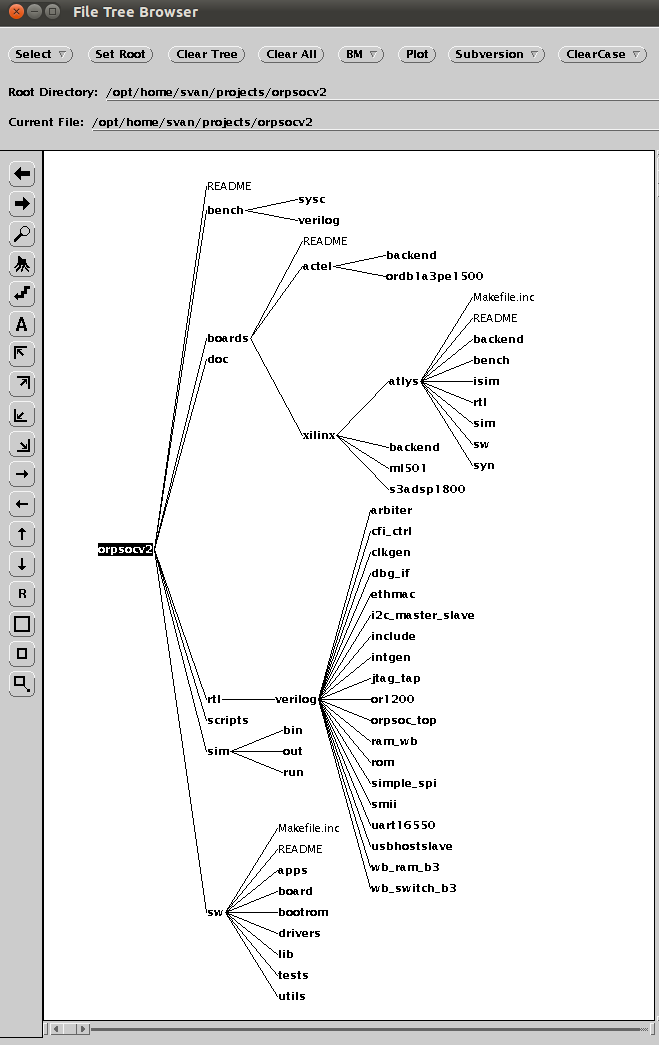
\includegraphics[width=0.8\textwidth,keepaspectratio=true]{./images/proyectoorpsoc}
  \caption{Esquema del Proyecto ORPSoC }
  \label{fig:esquema}
 \end{center}
\end{figure}

 \section{Instalación de herramientas}
 \subsection{Instalación de herramientas GNU}

Los programas deben ser instalados en el directorio / opt. Utilice los siguientes comandos para descomprimir y descomprimir el archivo descargado: 


 \section{Instalación de herramientas Xilinx}

Antes de realizar esto necesitamos tener instaladas correctamente las herramientas de Xilinix. Luego de la instalación debemos agregar al PATH de Linux las rutas a los binarios necesarios para realizar el proceso. 

\begin{lstlisting}[breaklines]
 usuario@usuario-desktop:~/$ source (ruta a Xilinx ISE)/settings32.sh  
\end{lstlisting}

 \section{Syntesis}
La construcción del proyecto está configurada para el uso de Makefiles. Los pasos a realizar son los siguientes:

\begin{itemize}
\item Los archivos necesarios para realizar la síntesis se encuentran en 

\begin{lstlisting}[breaklines]
(orpsoc_dir)/boards/xilinx/(board)/syn/
\end{lstlisting}

\item Limpiamos cualquier síntesis anteriormente realizada 
\begin{lstlisting}[breaklines]
usuario@usuario-desktop:(orpsoc_dir)/boards/xilinx/s3adsp1800/syn/xst/run$ make clean
\end{lstlisting}

\item Verificamos que solo existe el makefile
\begin{lstlisting}[breaklines]
usuario@usuario-desktop:(orpsoc_dir)/boards/xilinx/s3adsp1800/syn/xst/run$ ls

Makefile
\end{lstlisting}

\item Realizamos una nueva síntesis
\begin{lstlisting}[breaklines]
usuario@usuario-desktop:(orpsoc_dir)/boards/xilinx/s3adsp1800/syn/xst/run$ make all
\end{lstlisting}

\end{itemize} 

% #### Generating Xilinx PRJ file ####
% #### Generating XST file ####
% #### Generating Xilinx XCF file ####
% #### Running XST ####

\section{Place and Route}
%///////////// Place and Route ////////////////////////
Luego de la síntesis para realizar el procedimiento Place and Route (PAR) debemos ir a la carpeta
\begin{lstlisting}[breaklines]
(orpsoc_dir)/boards/xilinx/(board)/backend/par/
\end{lstlisting}
Limpiamos cualquier PAR anteriormente realizado

\begin{lstlisting}[breaklines]
usuario@usuario-desktop:(orpsoc_dir)/boards/xilinx/s3adsp1800/backend/par/run$ make clean
\end{lstlisting}

Verificamos que solo existe el makefile
\begin{lstlisting}[breaklines]
usuario@usuario-desktop:(orpsoc_dir)/boards/xilinx/s3adsp1800/backend/par/run$ ls
Makefile
\end{lstlisting}

Realizamos el proceso PAR 

\begin{lstlisting}[breaklines]
usuario@usuario-desktop:(orpsoc_dir)/boards/xilinx/s3adsp1800/backend/par/run$ make orpsoc.ncd
\end{lstlisting}
El reporte del PAR se encuentra en 
\begin{lstlisting}[breaklines]
usuario@usuario-desktop:(orpsoc_dir)/boards/xilinx/s3adsp1800/backend/par/run$ cat orpsoc.par
\end{lstlisting}

Para listar los valores de configuración con las que se esta realizando el proceso
\begin{lstlisting}[breaklines]
usuario@usuario-desktop:(orpsoc_dir)/boards/xilinx/s3adsp1800/backend/par/run$ make print-config
\end{lstlisting}

Para realizar un informe de "timing post place" 

\begin{lstlisting}[breaklines]
usuario@usuario-desktop:(orpsoc_dir)/boards/xilinx/s3adsp1800/backend/par/run$ make timingreport
\end{lstlisting}

El informe se encuentra en:

\begin{lstlisting}[breaklines]
usuario@usuario-desktop:(orpsoc_dir)/boards/xilinx/s3adsp1800/backend/par/run$ cat orpsoc.twr | less
\end{lstlisting}


 \section{Generación del .Bit}

Finalmente generamos el bitfile que contiene la configuración que debemos cargar en la FPGA.

\begin{lstlisting}[breaklines]
usuario@usuario-desktop:(orpsoc_dir)/boards/xilinx/s3adsp1800/backend/par/run$ make orpsoc.bit
\end{lstlisting}

 \section{Configuración de la FPGA}

%//////////// XC3SPROG INSTALLATION   //////////////
Para descargar el bitfile de configuración utilizamos xc3sprog y un programador basado en FTDI2232. Este hardware requiere de la herramienta 

Descargamos el código del programa
\begin{lstlisting}[breaklines]
usuario@usuario-desktop:~/$ svn checkout svn://svn.code.sf.net/p/xc3sprog/code/trunk xc3sprog-code
usuario@usuario-desktop:~/$ cd xc3sprog-code
usuario@usuario-desktop:~/$   
\end{lstlisting}
%........   TERMINAR PROCESO DE COMPILACIÓN ..... 


%//////////// DOWNLOAD THE BITSTREAM ON FPGA   //////////////

Luego de conectar el programador en el conector J4. Chequeamos el funcionamiento escaneando la cadena JTAG
\begin{lstlisting}[breaklines]
usuario@usuario-desktop:~$ sudo (ruta a xc3sprog)/xc3sprog  -c ftdi -j
usuario@usuario-desktop:(orpsoc_dir)/boards/xilinx/s3adsp1800/backend/par/run$ sudo (ruta a xc3sprog)/xc3sprog  -c ftdi  orpsoc.bit 
\end{lstlisting}

 \section{Descarga del BITSTREAM a la SPI }

%//////////// DOWNLOAD THE BITSTREAM ON SPI   //////////////
Inicialmente descargamos el bitfile provisto en la carperta
\begin{lstlisting}[breaklines]
xc3sprog/bscan_files
\end{lstlisting} 
 que configura la fpga para actuar como intermediario ante la FLASH SPI y así lograr grabar en la misma.
\begin{lstlisting}[breaklines]
usuario@usuario-desktop:(orpsoc_dir)/boards/xilinx/s3adsp1800/backend/par/run$ sudo (ruta a xc3sprog)/xc3sprog  -c ftdi (ruta a xc3sprog)/bscan_spi/xc3sd1800-fg676.bit 
\end{lstlisting} 

Ahora podemos descargar el bitstream a la FLASH SPI mediante 
\begin{lstlisting}[breaklines]
usuario@usuario-desktop:(orpsoc_dir)/boards/xilinx/s3adsp1800/backend/par/run$ sudo (ruta a xc3sprog)/xc3sprog  -c ftdi  -I orpsoc.bit 
\end{lstlisting}
 \newpage
 
\chapter{Códigos de Prueba}

 \section{Introducción}

En el presente anexo se  publicaran los corresppndientes códigos que se realizaron con el fin de probar el correcto funcionamiento de los requerimientos e los diferentes prototipos


 \section{Programa de Prueba para el UART}

\begin{lstlisting}[language=C,frame=single]
#include <board.h>
#include <support.h>
#include <or1200.h>
#include <int.h>

#include <uart.h>

int main()
{
	uart_init();
	int_init();
	int_add(UART_IRQ, &uart_interrupt, NULL);
	
	/* We can't use printf because in this simple example
	   we don't link C library. */
	uart_print_str("Hello World.\n");
	
	report(0xdeaddead);
	or32_exit(0);
}

\end{lstlisting}

 \section{Programa de Prueba para Ethernet}

\begin{lstlisting}[language=C,frame=single]
#include <board.h>
#include <support.h>
#include <or1200.h>
#include <int.h>

#include <uart.h>
#include <eth.h>


extern int eth_rx_len;
extern int eth_rx_done, eth_tx_done;
extern unsigned char * eth_rx_data;
extern unsigned char * eth_tx_data;

void eth_receive()
{
	int i;
	uart_print_str("Length: \n");
	uart_print_long(eth_rx_len);
	uart_print_str("\n");
	uart_print_str("Data: \n");
	for ( i = 0; i < eth_rx_len; i++ )
	{
		uart_print_short(eth_rx_data[i]);
		uart_print_str("\n");
	}
	eth_recv_ack();
}

int main()
{
	uart_init();

	int_init();
	eth_init();
	int_add(UART_IRQ, &uart_interrupt, NULL);
	int_add(ETH_IRQ, &eth_interrupt, NULL);

	/* We can't use printf because in this simple example
	   we don't link C library. */
	uart_print_str("Hello World.\n");

	eth_tx_data[0] = 0xFF;
	eth_tx_data[1] = 0x2B;
	eth_tx_data[2] = 0x40;
	eth_tx_data[3] = 0x50;

	eth_send(4);

	while(1)
	{
		if (eth_rx_done)
		{
			eth_receive();
		}
	}

	report(0xdeaddead);
	or32_exit(0);
}
\end{lstlisting}


 \section{Programa de Prueba para Capacidad de Procesamiento}

\begin{lstlisting}[language=C,frame=single]
#include <board.h>
#include <support.h>
#include <or1200.h>
#include <int.h>
#include <uart.h>

#define con 15
#define N 16

void genmatriz(unsigned seed1,unsigned *matriz,int indice){
/*
    uart_print_str("seed ="); 
    uart_print_long(seed1);
    uart_print_str("\n");
*/    
    unsigned sr1[N] ;
    unsigned i , j ,q  ;
    unsigned tmp;    
    
    for(i=0; i<N; i++){
  	sr1[i] =  (seed1&1);
  	seed1/=2;
    }

    for (q=0;q<(indice*indice);q++){
		tmp = sr1[15]^sr1[14]^sr1[13]^sr1[11];
		
		for(j=N;j>0;j--) sr1[j]=sr1[j-1];
		sr1[0] = tmp;

		matriz[q] = tmp;
		
                //uart_print_long(tmp);
		//if (((q+1)%con_i)==0) uart_print_str("\n");
    }   

}


int main()
{
 
    // Declaraciones
    int i , j , k ; 
    int indice;
    unsigned matriz  [con*con];
    unsigned matrizA [con*con];
    unsigned matrizB [con*con];
    
    int producto ; 
    int acumulador ;
    unsigned tiempo;
    int useg;

	

////// Setup Inicial
    //tick_init();
    asm("l.mtspr\t\t%0,%1,0": : "r" (SPR_TTMR), "r" (SPR_TTMR_CR));
    asm("l.mtspr\t\t%0,%1,0": : "r" (SPR_TTCR), "r" (0x0));
    //mtspr(SPR_TTCR, SPR_TTMR_CR);
    //mtspr(SPR_TTCR, 0x0);
        
    //tick_start();
    asm("l.mtspr\t\t%0,%1,0": : "r" (SPR_TTCR), "r" (0x0));
    //mtspr(SPR_TTCR, 0x0);
    
    tiempo = mfspr(SPR_TTCR);
    useg = (int) tiempo * 50 ;
    uart_print_str("Tick de ejecucion setup tick :");
    uart_print_long((long)tiempo);
    uart_print_str(" En us = ");
    uart_print_long(useg);
    uart_print_str("\n");   
   
    for (indice=1; indice<=con; indice++){
    //tick_start();
    //asm("l.mtspr\t\t%0,%1,0": : "r" (SPR_TTCR), "r" (0x0));
    //uart_print_str("Matrices de  :");
    uart_print_long(indice);
    uart_print_str(",");
    //uart_print_str("\n");

 
    mtspr(SPR_TTCR, 0x0);
    
    i= 0;
    j= 0;
    k= 0;
    producto = 0;
    acumulador = 0;
/*
    for (i=0;i<indice;i++){
		for (j=0;j<indice;j++){
			matriz  [i][j] = 0;
			matrizA [i][j] = 1;
			matrizB [i][j] = 1;
		}
	}
*/
      tiempo = mfspr(SPR_TTCR);
      genmatriz (tiempo,matriz,indice);
      tiempo = mfspr(SPR_TTCR);
      genmatriz (tiempo,matrizA,indice);
      tiempo = mfspr(SPR_TTCR);
      genmatriz (tiempo,matrizB,indice);
    

//    tiempo = mfspr(SPR_TTCR);
//    useg = (int) tiempo * 50 ; 
//    uart_print_str("Tick de ejecucion seteo de variables :");
//    uart_print_long((long)tiempo);
//    uart_print_str(" En us = ");
//    uart_print_long(useg);
// 	uart_print_str("\n");
 	 
 
	mtspr(SPR_TTCR, 0x0);
    
	for (i=0;i<indice;i++){
		for (j=0;j<indice;j++){
			for (k=0;k<indice;k++){
				producto = matrizA[i*con+k] * matrizB[k*con+j];
				acumulador = acumulador + producto;
			}
			matriz [i*con+j] = acumulador;
			acumulador = 0;
		}	
	}
    
    tiempo = mfspr(SPR_TTCR);
//    useg = (int) tiempo * 50 ;
//    uart_print_str("Tick de ejecucion de la multiplicacion :");
    uart_print_long((long)tiempo);
//    uart_print_str(" En us = ");
//    uart_print_long(useg);
    uart_print_str("\n");   
    

/*
    uart_print_str("Matriz Resultado");   
    uart_print_str("\n");   
    
    for (i=0;i<indice;i++){
		for (j=0;j<indice;j++){
			uart_print_long(matriz [i*con+j]);
			uart_print_str(" ");
		}
		uart_print_str("\n");
	}
  
 */  
    } 
  
    uart_print_str("Fin del programa\n");

    return 0;
}
\end{lstlisting}

 \subsection{Generador de secuencia binaria seuda aleatoria}
\begin{lstlisting}[language=C,frame=single]
#include "stdio.h"
#include "time.h"
#define con_i 10

#define N 16

void genmatriz(unsigned seed1,unsigned *matriz){
    printf ("seed1 ="); 
    printf("%x",seed1);
    printf("\n");   
    
    //unsigned  seed1 ; 
    unsigned sr1[N] ;
    unsigned i , j ,q  ;
    unsigned tmp;    
    
    for(i=0; i<N; i++){
  	sr1[i] =  (seed1&1);
  	seed1/=2;
    }

    for (q=0;q<(con_i*con_i);q++){
		tmp = sr1[15]^sr1[14]^sr1[13]^sr1[11];
		
		for(j=N;j>0;j--) sr1[j]=sr1[j-1];
		sr1[0] = tmp;

		matriz[q] = tmp;
		
                //printf ("%i ",tmp);
		//if (((q+1)%con_i)==0) printf ("\n");
    }   
	printf ("\n\n");
}

int main(void ) {

unsigned matriz[100] ;
unsigned i,j ;
genmatriz (time(NULL),matriz);
for (i=0;i<100;i++){
	printf ("%i ",matriz[i]);
	if (((i+1)%10)==0) printf ("\n");
}

 return 0;
}
\end{lstlisting}

 \section{Programa de Prueba de SDRAM}
 \begin{lstlisting}[language=C,frame=single]
 #include "cpu-utils.h"
#include "board.h"
#include "sdram.h"
#include "uart.h"
#include "printf.h"

#ifndef _SDRAM_H_
#define _SDRAM_H_

#ifdef  MT48LC32M16A2 // 64MB SDRAM part
#define SDRAM_SIZE 0x04000000
#define SDRAM_ROW_SIZE 2048 // in bytes (10 bits col addr, 2 bytes per)
#define SDRAM_NUM_ROWS_PER_BANK (8192) // 13-bit row address
#define SDRAM_NUM_BANKS 4
#endif

#ifdef  MT48LC16M16A2 // 32MB SDRAM part
#define SDRAM_SIZE 0x02000000
#define SDRAM_ROW_SIZE 1024 // in bytes (9 bits col addr, 2 bytes per)
#define SDRAM_NUM_ROWS_PER_BANK (8192) // 13-bit row address
#define SDRAM_NUM_BANKS 4
#endif

#ifdef MT48LC4M16A2 // 8MB SDRAM part
#define SDRAM_SIZE 0x800000
#define SDRAM_ROW_SIZE 512 // in bytes (8 bits col addr, 2 bytes per)
#define SDRAM_NUM_ROWS_PER_BANK (4096) // 12-bit row address
#define SDRAM_NUM_BANKS 4
#endif


#endif


#define SDRAM_NUM_ROWS (SDRAM_NUM_ROWS_PER_BANK * SDRAM_NUM_BANKS)

#define START_ROW 128

int main()
{

  uart_init(DEFAULT_UART);


  printf("\n\tSDRAM rows test\n");

  printf("\n\tWriting\n");
  
  int i; // Skip first 64KB, code/stack resides there - TODO determine this from
  // stack linker variable!
  for(i=START_ROW;i<(SDRAM_NUM_ROWS);i++)
    {
      REG32((i*(SDRAM_ROW_SIZE))) = i;
      printf("\r\t0x%x", i);
    }

  printf("\n\tReading\n");

  int read_result = 0;

  for(i=START_ROW;i<(SDRAM_NUM_ROWS);i++)
    {
      printf("\r\t0x%x", i);
      read_result = REG32((i*(SDRAM_ROW_SIZE)));
      if (read_result != i)
	{
	  printf("\n\Error at 0x%x, read 0x%x, expected 0x%x\n",
		 (i*SDRAM_ROW_SIZE), read_result, i);
	  report(0xbaaaaaad);
	  report(i);
	  report(read_result);
	  exit(0xbaaaaaad);
	}
    }
  printf("\n\tTest OK.\n");
  exit(0x8000000d);  
}
 
 \end{lstlisting}

 \section{Programa de Prueba Ethernet del Proyecto ORPSoC}
 \begin{lstlisting}[language=C,frame=single]
 
int main ()
{
  
	print_packet_contents = 0; // Default to not printing packet contents.
	packet_inspect_debug = 0;
	print_ethmac_debug_reg = 0;

	/* Initialise vector handler */
	int_init();

	/* Install ethernet interrupt handler, it is enabled here too */
	int_add(ETH0_IRQ, oeth_interrupt, 0);

	/* Enable interrupts */
	cpu_enable_user_interrupts();
    
	last_char=0; /* Variable init for spin_cursor() */
	next_tx_buf_num = 4; /* init for tx buffer counter */

	uart_init(DEFAULT_UART); // init the UART before we can printf
	printf("\n\teth ping program\n\n");
	printf("\n\tboard IP: %d.%d.%d.%d\n",our_ip[0]&0xff,our_ip[1]&0xff,
	       our_ip[2]&0xff,our_ip[3]&0xff);
  
	ethmac_setup(); /* Configure MAC, TX/RX BDs and enable RX and TX in 
			   MODER */
  
	//scan_ethphys(); /* Scan MIIM bus for PHYs */
	//ethphy_init(); /* Attempt reset and configuration of PHY via MIIM */
	//ethmac_scanstatus(); /* Enable scanning of status register via MIIM */

	/* Loop, monitoring user input from TTY */
	while(1)  
	{
		char c;
      
		while(!uart_check_for_char(DEFAULT_UART))
		{
			
			spin_cursor();
			
			if (print_ethmac_debug_reg)
				oeth_print_wbdebug();
		}
      
		c = uart_getc(DEFAULT_UART);

		if (c == 's')
			tx_packet((void*) ping_packet, 98);
		else if (c == 'S')
			tx_packet((void*)big_ping_packet, 1514);
		else if (c == 'h')
			scan_ethphys();
		else if (c == 'i')
			ethphy_init();
		else if (c == 'c')
			oeth_ctrlmode_switch();
		else if (c == 'P')
		{
			print_packet_contents = print_packet_contents ? 0 : 1;
			if (print_packet_contents)
				printf("Enabling packet dumping\n");
			else
				printf("Packet dumping disabled\n");
		}
		else if (c == 'p')
			oeth_printregs();
		else if (c == 'a')
			ethphy_print_status(ethphy_found);
		else if (c >= '0' && c <= '9')
			scan_ethphy(c - 0x30);
		else if (c == 'r')
		{
			ethphy_reset(ethphy_found);
			printf("PHY reset\n");
		}
		else if (c == 'R')
		{
			//oeth_reset_tx_bd_pointer();
			ethmac_setup();
			printf("MAC reset\n");
		}
		else if (c == 'n')
			ethphy_reneg(ethphy_found);
		else if (c == 'N')
			ethphy_toggle_autoneg(ethphy_found);
		else if (c == 'm')
			ethmac_togglehugen();
		else if (c == 't')
			ethphy_set_10mbit(ethphy_found);
		else if (c == 'H')
			ethphy_set_100mbit(ethphy_found);
		else if ( c == 'b' )
		{
			printf("\n\t---\n");
			oeth_dump_bds();
			printf("\t---\n");
		}
      
		else if ( c == 'B' )
		{
			tx_packet((void*) broadcast_ping_packet, 298);
		}
		else if (c == 'u' )
			oeth_transmit_pause();
		else if (c == 'd' )
		{
			oeth_print_wbdebug();
			print_ethmac_debug_reg = !print_ethmac_debug_reg;
		}
		else if (c == 'D')
		{
			marvell_phy_toggle_delay();
		}
		else if (c == 'v' )
		{
			if (packet_inspect_debug)
				printf("Disabling ");
			else 
				printf("Enabling ");
			
			printf("packet type announcments\n");
			
			packet_inspect_debug = !packet_inspect_debug;
		}
		else if ( c == 'o' )
			oeth_toggle_promiscuous();
		else if (c == 'L')
			ethphy_toggle_loopback();
		else if (c == 'g')
			ethphy_toggle_gigadvertise();

	}
	 \end{lstlisting}
	 
	  \section{Programa de Prueba de Compilador y Depurador para ORPSoC - Números Primos}
 \begin{lstlisting}[language=C,frame=single]
Código de prueba de numeros primos 
	 \end{lstlisting}
	
 \newpage

 %\chapter{MANUAL DE USUARIO: INTERFAZ GRAFICA}
 %\input{manual_gui}          